
\section{Introduction to Semiconductors}
Semiconductors are materials that possess electrical conductivity between that of conductors and insulators. Their conductivity can be controlled by introducing impurities or applying electric fields, making them essential for modern electronics.

\subsection*{Gallium Arsenide (GaAs)}
\textbf{Properties:}
\begin{itemize}
    \item High electron mobility, allowing faster operation.
    \item Superior performance at high frequencies compared to silicon.
\end{itemize}

\textbf{Applications:}
\begin{itemize}
    \item Used in microwave circuits, high-speed data communication, and satellite systems.
\end{itemize}

\subsection*{N-Type and P-Type Semiconductors}
Semiconductors can be classified into:
\begin{itemize}
    \item \textbf{N-Type:} Formed by adding donor impurities that introduce free electrons as majority carriers.
    \item \textbf{P-Type:} Formed by adding acceptor impurities that create holes (absence of electrons) as majority carriers.
\end{itemize}

\textbf{Illustration of N-Type and P-Type Materials:}

\begin{center}
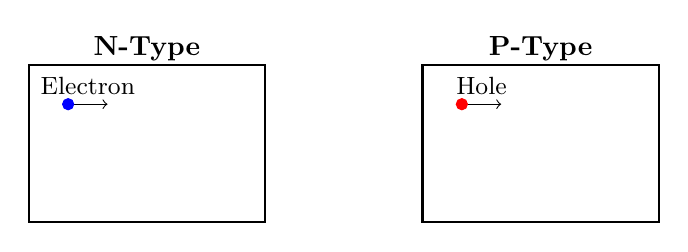
\begin{tikzpicture}
% N-type material
\draw[thick] (0, 0) rectangle (3, 2);
\draw[->] (0.5, 1.5) -- (1, 1.5) node[midway, above] {\small Electron};
\filldraw[blue] (0.5, 1.5) circle (2pt);
\node at (1.5, 2.2) {\textbf{N-Type}};
% P-type material
\draw[thick] (5, 0) rectangle (8, 2);
\draw[->] (5.5, 1.5) -- (6, 1.5) node[midway, above] {\small Hole};
\filldraw[red] (5.5, 1.5) circle (2pt);
\node at (6.5, 2.2) {\textbf{P-Type}};
\end{tikzpicture}
\end{center}

\section*{PN-Junction Diodes}
A PN-junction diode consists of a junction formed by combining N-type and P-type materials. The behavior of a diode depends on the applied bias voltage.

\subsection*{Forward Bias}
When the P-side is connected to a positive voltage, the depletion region narrows, allowing current flow.

\subsection*{Reverse Bias}
When the P-side is connected to a negative voltage, the depletion region widens, preventing current flow.

\textbf{Diagram of Forward and Reverse Bias:}

\begin{center}
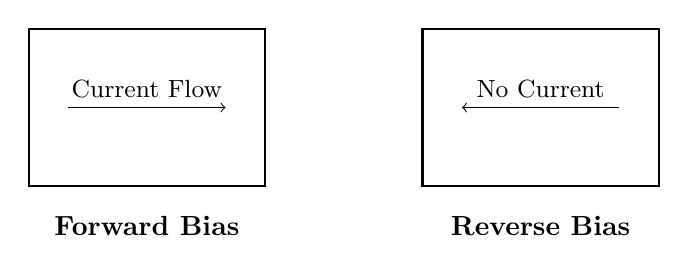
\begin{tikzpicture}
% Forward bias
\draw[thick] (0, 0) rectangle (3, 2);
\draw[->] (0.5, 1) -- (2.5, 1) node[midway, above] {\small Current Flow};
\node at (1.5, -0.5) {\textbf{Forward Bias}};
% Reverse bias
\draw[thick] (5, 0) rectangle (8, 2);
\draw[<-] (5.5, 1) -- (7.5, 1) node[midway, above] {\small No Current};
\node at (6.5, -0.5) {\textbf{Reverse Bias}};
\end{tikzpicture}
\end{center}

\section*{Bipolar Junction Transistors (BJTs)}
A BJT consists of three layers: emitter, base, and collector. It is classified as NPN or PNP based on the arrangement of the layers.

\subsection*{Operation}
\begin{itemize}
    \item \textbf{NPN Transistor:} Current flows when the base-emitter voltage exceeds 0.6V.
    \item \textbf{PNP Transistor:} Operates similarly but with opposite polarities.
\end{itemize}

\textbf{Key Parameter:} The current gain, $\beta$, is the ratio of collector current to base current.

\textbf{Diagram of NPN Transistor Operation:}

\begin{center}
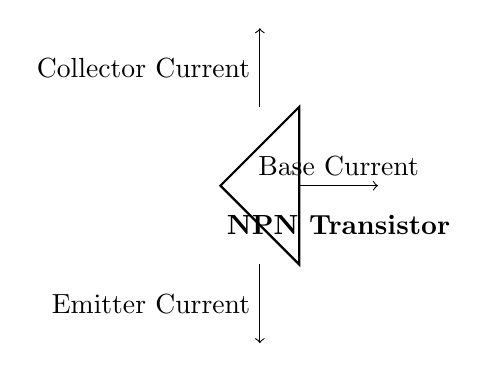
\begin{tikzpicture}
% Transistor diagram
\draw[thick] (0, 0) -- (1, 1) -- (1, -1) -- cycle;
\draw[->] (1, 0) -- (2, 0) node[midway, above] {Base Current};
\draw[->] (0.5, 1) -- (0.5, 2) node[midway, left] {Collector Current};
\draw[->] (0.5, -1) -- (0.5, -2) node[midway, left] {Emitter Current};
\node at (1.5, -0.5) {\textbf{NPN Transistor}};
\end{tikzpicture}
\end{center}

\section*{Field-Effect Transistors (FETs)}
FETs are controlled by an electric field applied to the gate terminal.

\subsection*{Types of FETs}
\begin{itemize}
    \item \textbf{Junction FETs (JFETs):} Simple structure with high input impedance.
    \item \textbf{MOSFETs:} Versatile devices available in depletion and enhancement modes.
\end{itemize}

\textbf{Diagram of a MOSFET:}

\begin{center}
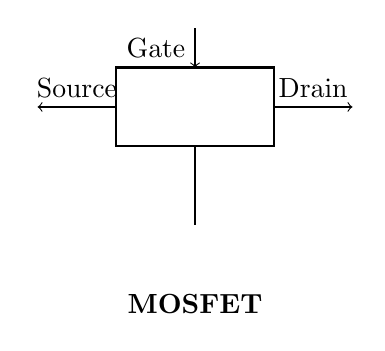
\begin{tikzpicture}
% MOSFET diagram
\draw[thick] (0, 0) rectangle (2, 1);
\draw[thick] (1, 0) -- (1, -1);
\draw[->] (2, 0.5) -- (3, 0.5) node[midway, above] {Drain};
\draw[<-] (-1, 0.5) -- (0, 0.5) node[midway, above] {Source};
\draw[->] (1, 1.5) -- (1, 1) node[midway, left] {Gate};
\node at (1, -2) {\textbf{MOSFET}};
\end{tikzpicture}
\end{center}

\section*{Protective Measures for MOSFETs}
Zener diodes are often connected to the gate of a MOSFET to protect against voltage spikes caused by static discharge.

\section*{High-Frequency Applications}
Gallium arsenide is the material of choice for high-frequency and microwave applications due to its superior performance compared to silicon.

\section*{Glossary of Key Terms}
\begin{itemize}
    \item \textbf{Acceptor Impurity:} Adds holes to the crystal structure, creating P-type material.
    \item \textbf{Depletion Region:} The region in a PN junction where charge carriers are depleted, acting as an insulator.
    \item \textbf{Beta ($\beta$):} The ratio of collector current to base current in a BJT.
\end{itemize}

\end{document}
